\documentclass[letterpaper,10pt]{article}

\usepackage{titling}
\usepackage{listings}
\usepackage{url}
\usepackage{setspace}
\usepackage{subfig}
\usepackage{sectsty}
\usepackage{pdfpages}
\usepackage{colortbl}
\usepackage{multirow}
\usepackage{multicol}
\usepackage{relsize}
\usepackage{amsmath}
\usepackage{wasysym}
\usepackage{fancyvrb}
\usepackage{amssymb}
\usepackage{ifsym}
\usepackage{amsmath,amssymb,amsthm,graphicx,xspace}
\usepackage[titlenotnumbered,noend,noline]{algorithm2e}
\usepackage[compact]{titlesec}
\usepackage{XCharter}
\usepackage[T1]{fontenc}
\usepackage{tikz}
\usetikzlibrary{arrows,automata,shapes,trees,matrix,chains,scopes,positioning,calc}
\tikzstyle{block} = [rectangle, draw, fill=blue!20, 
    text width=2.5em, text centered, rounded corners, minimum height=2em]
\tikzstyle{bw} = [rectangle, draw, fill=blue!20, 
    text width=4em, text centered, rounded corners, minimum height=2em]

\definecolor{namerow}{cmyk}{.40,.40,.40,.40}
\definecolor{namecol}{cmyk}{.40,.40,.40,.40}

\let\LaTeXtitle\title
\renewcommand{\title}[1]{\LaTeXtitle{\textsf{#1}}}


\newcommand{\handout}[5]{
  \noindent
  \begin{center}
  \framebox{
    \vbox{
      \hbox to 5.78in { {\bf ECE356: Database Systems } \hfill #2 }
      \vspace{4mm}
      \hbox to 5.78in { {\Large \hfill #4  \hfill} }
      \vspace{2mm}
      \hbox to 5.78in { {\em #3 \hfill} }
    }
  }
  \end{center}
  \vspace*{4mm}
}

\newcommand{\lecture}[3]{\handout{#1}{#2}{#3}{Lecture #1}}
\newcommand{\tuple}[1]{\ensuremath{\left\langle #1 \right\rangle}\xspace}

\addtolength{\oddsidemargin}{-1.000in}
\addtolength{\evensidemargin}{-0.500in}
\addtolength{\textwidth}{2.0in}
\addtolength{\topmargin}{-1.000in}
\addtolength{\textheight}{1.75in}
\addtolength{\parskip}{\baselineskip}
\setlength{\parindent}{0in}
\renewcommand{\baselinestretch}{1.5}
\newcommand{\term}{Winter 2018}

\singlespace


\begin{document}

\lecture{ 26 --- Snapshot Isolation, Weak Consistency, Insert/Delete }{\term}{Jeff Zarnett}

\section*{Snapshot Isolation for Concurrency Control}

We already got a look at the idea of transaction isolation but we are now going to examine more carefully how it works behind the scenes. In general, the idea is that every transaction has its own ``world'' it can operate in and then we need to merge the result when the transaction is ready to commit. And that needs to be done atomically.

We can use validation to decide whether a transaction is allowed to commit. This applies really only for transactions that do at least one write. Reads don't interfere with one another, really, and if the two writes are on disjoint items, there are no problems there either. It only gets interesting if there are two transactions that have items in common that run at the same time. Remember that here, when we talk about concurrency, we mean two transactions that are ``active'' at the same time.

Usually, we do not like to just allow both transactions to go forward because the first write is then overwritten by the second; a ``lost update''~\cite{dsc}. This is sometimes  acceptable as a choice, even if some textbooks say that this is really undesirable and horrible.

The first snapshot isolation strategy is called \textit{first committer wins}: whichever transaction $T$ is ready to commit first has to pass a simple test. If any transaction concurrent with $T$ has already written an update to any data item that $T$ wants to write, $T$ is rolled back; otherwise $T$ commits and its updates are written to the database. It's called first committer wins, because whatever transaction gets to the commit statement proceeds and any later transactions are rolled back.

The alternative is \textit{first updater wins} and this is pretty much exactly what it sounds like: it is the timing of the write rather than the timing of the commit that indicates which transaction is allowed to proceed and which one(s) must be rolled back.  

Locks are always released when the transaction either commits or aborts as is necessary. But strangely, the fact that a transaction $T_{2}$ writes a value later than $T_{1}$ writes that same value might succeed if for some other reason the first transaction aborts~\cite{dsc}. But to keep things from getting rather confusing it is likely a simple implementation will just force the abort if $T_{2}$ finds it wants to get a write lock on a data item that is currently exclusively held. Failure equals death indeed.

This scheme as presented, however, does not ensure serializability. There are two suggested scenarios for how this might happen~\cite{dsc}:

Example 1: If we have two concurrent transactions $T_{1}$ and $T_{2}$ that operate on $A$ and $B$. If $T_{1}$ reads $A$ and $B$, then updates $B$ and $T_{2}$ reads $A$ and $B$ and updates $A$, we have the potential for a conflict. Neither transaction sees the updates of the other when they do their reads, when it comes to the write... well... neither one has a problem, strictly speaking, because they write different data items and whether first-updater-wins or first-committer-wins takes place, neither transaction is detected as conflicting and neither is rolled back.

In spite of that, we have a problem: we have an outcome (output data) that could not happen if we had serial execution of the transactions; either $T_{1}$ then $T_{2}$ or $T_{2}$ then $T_{1}$. Now what? 

It looks like under this scheme, some things like foreign key checks, primary key checks, et cetera, cannot be checked in the transaction world itself and must be checked an extra time when the transaction commits and is finally ready to replace the actual stored version on the database.

Example 2: Imagine we still have $T_{1}$ and $T_{2}$ and $A$ and $B$ as before. $T_{1}$ reads $B$ and updates $B$, and $T_{2}$ reads $A$ and $B$ and updates $A$. As before, there are no direct conflicts on the data items so neither first-committer-wins nor first-updater-wins would detect a problem. Furthermore, there's a possible serial order here: there are no conflicts on $A$, and no cycle in the precedence graph: $T_{2}$ reads the value of $B$ that existed before the write by $T_{1}$. 

A third transaction, even one that is read-only, can cause the cycle to occur, however. If $T_{1}$ commits and $T_{2}$ is still running, and $T_{3}$ is created and its view of the world has the update from $T_{1}$ but not $T_{2}$ and suddenly we have the cycle in the precedence graph, rendering the schedule non-serializable.

After all that, though, we can accept some degree of non-serializability as long as it does not produce inconsistent results. For performance and other reasons it might be sensible to just let execution orders that are not serializable proceed as long as they don't produce inconsistent results.  Or we will allow such things if we are convinced that inconsistencies don't make a big difference. 

A small example of when we might have to really enforce constraints is the primary key. If you have a sequential counter of some sort, an ID number, then two newly created entries in the database would each be looking at the old snapshot data and will produce the same new number. Neither transaction can detect that another has tried to use the same ID number, but only when we are actually ready to perform the second commit will the duplicate key value be detected.

This is, actually, slightly different from what we have discussed thus far, because it focuses on an insertion rather than just a simple write. That is different...

\section*{Changes: Insertion \& Deletion}

If you can believe it, all the discussion thus far on the subject of concurrency control has excluded the possibility of performing an insertion or deletion on the data items; only read and writes were allowed. But those are pretty important operations, so we can't ignore them forever. 

\paragraph{Deletion.} The impact of delete depends, obviously, on what the else is going on at the time. We can take a view of what happens by considering the relation of the delete instruction relative to other instructions. In each of the cases, instruction $I_{1}$ is our delete instruction~\cite{dsc}:

\begin{itemize}
	\item \textbf{Read instruction}: If the delete $I_{1}(X)$ happens before a read of X then the read will get a logical error; if the read happens before the delete, there is no problem.
	\item \textbf{Write Instruction}: If the delete happens before the write, the write will get a logical error; if the write happens before the delete, there is no problem.
	\item \textbf{Delete Instruction}: Whichever instruction goes first will succeed; the second one will have an error (can't delete a deleted item).
	\item \textbf{Insert Instruction}: If the element doesn't exist to begin with, the delete can't be before the insert, otherwise there's nothing to delete... If the item did exist then a delete should go first so the new item replaces it.
\end{itemize}

It is sensible to conclude that the delete operation requires an exclusive lock on that data item before it can be deleted. Also, the rules for writing apply for a deletion action if using a timestamp ordering protocol. It is probably not a stretch to imagine it is very much like a write.

\paragraph{Insertion.} The insert operation conflicts were explained above when discussing deletion, so they don't need to be repeated here. Insert is also a lot like a write so again, the insert operation is treated like a write: the newly created item is treated as exclusively locked by its creating transaction until the transaction commits~\cite{dsc}.

I think it bears repeating at this level that the changes we want to make here are at the level of actual manipulation of the underlying data. It is perfectly valid, from the perspective of the user writing the SQL, to do a read and get back ``no results'' because the item was very recently deleted. The problem here is that we have identified what data elements we need to access and the ones we want are not there (or not as expected, or there are extra ones...) and we need to stop, go back, reformulate the list of things to do, and then try to do it again. 

\paragraph{The Phantom of the Op... Database.} Suppose the following transactions are executed concurrently: (1) a select statement that finds all books published by author ``Jim Butcher''; (2) an insert statement that adds a new book with author ``Jim Butcher'' amongst its attributes. 

There are two possibilities for how this might go: $T_{1}$ happens before $T_{2}$ or vice versa. If $T_{2}$ happens first, nothing weird happens -- in the serial schedule, first it's $T_{2}$ then $T_{1}$ and the new book appears in the results. In the second case, if $T_{1}$ goes first and it does not contain the new book, then in the serial schedule, $T_{1}$ appears first.... except... these transactions do not operate on any tuples in common and yet there is still some dependencies between them, and they conflict on a ``phantom'' tuple (one that doesn't exist)~\cite{dsc}. This is called the \textit{Phantom Phenomenon} and has nothing at all to do with the breakout success of the Andrew Lloyd Webber musical. 

The phantom phenomenon can also happen if a read changes the value, say, if an item was entered incorrectly as ``Jim Butchr'', a corrective update statement run at the same time as $T_{1}$ above produces the same problem.

As a first solution, you might consider that an insertion or deletion should exclusively lock the relation entirely. That's one way to do it, it's certainly likely to be effective at getting rid of the phantom problem, but it is a painful solution because it forces a lot of transactions to wait or roll back when we really don't need that. The goal is to prevent insertions and updates that match the predicate in question, but only those (keeping the scope of the lock as minimal as possible)

Remember the index? So far we have just assumed that data items being updated are tuples, but that's not strictly true, because index data elements are also data and need to be lockable. Finding items that match a search predicate requires searching an index or performing a full table scan to find the data~\cite{dsc}. 

Idea: let's associate a data item (available to be locked) with each table, with the goal that it represents the way to find tuples in the relation~\cite{dsc}. Any time we want to update the data about what is in the relation, and transactions that want to read what tuples are in the relation need to also lock this item (in shared mode perhaps). And anything that operates on an index must lock the index. This moves the lock out of the realm of shadows and into the ``real'' world -- the lock conflicts here are now on an actual lock item.

Keep in mind this is very much distinct from locking the entire table: locking is still required on tuples and holding this sort of lock only restricts whether other transaction can update (or read) the information about what tuples are in the relation~\cite{dsc}. Even so, it's not all that dissimilar from the idea of having one lock for the whole table, in that it almost serializes all transactions.

An alternative is \textit{index locking}, which allows us to lock parts of the index at finer granularity. The protocol is~\cite{dsc}:

\begin{itemize}
	\item Every relation must have at least one index.
	\item A transaction $T_{i}$ can only access tuples after it has found them using an index (if we must do a full table scan, it's treated as if we just crawled through the whole of some index...)
	\item A transaction that performs a lookup (finding one tuple or multiple) must get a shared lock on all the index leaf nodes it accesses.
	\item A transaction may not insert, delete, or update any tuples in the relation without updating every index of that relation. That requires getting exclusive locks on all index leaf nodes affected by the operation. 
	\item Locks are still obtained on tuples as usual.
	\item Two phase locking protocol still must be followed. 
\end{itemize}


\paragraph{Predicate Locking.} You may imagine that the idea of index locking does not actually match very well with the idea of making the locking match the predicates only, such as only checking on things that affect author. That sort of locking technique sounds good but it is more difficult to implement. 

\subsection*{Weak Consistency}

The SQL standard provides several isolation levels, and it's not necessary that we stick with serializability as the level of consistency we are willing to accept. We can weaken the rules a bit to get some more performance out of the database and that gives us what is called \textit{weak consistency}: there are rules, but they are more like... guidelines?

\paragraph{Degree-Two Consistency.}
The idea of \textit{degree-two consistency} is to prevent cascading rollbacks (aborts) without guaranteeing serializability. There are shared and exclusive locks, but two-phase behaviour is not required; in fact shared locks can be released at any time and locks can be acquired at any time, but exclusive locks must be held until the transaction commits or aborts~\cite{dsc}. This means that we might read out of date data, but uncommitted values can never be read, so the level of transaction isolation here is ``read-committed''.

\paragraph{Cursor Stability.} Cursor stability is a form of degree-two consistency for programs that iterate over some set of tuples using an iterator or cursor~\cite{dsc}. This means that the tuples are examined or processed one at a time, in some order. To make sure that this works alright, the tuple currently being examined needs to be locked: before processing it is locked in shared mode; if any processing changes that tuple then it must first be locked in exclusive mode. 

We don't get serializability of the transactions, but it can be a way to improve performance in a database where there are a number of relations that are popular and frequently accessed. But ultimately this offloads some of the work onto the applications using the database, meaning they must make sure they don't have a problem with non-serializable schedules~\cite{dsc}.

\paragraph{Users Ruin Everything...}
Remember the example earlier about selecting seats on a flight (or at a concert or sporting event...). When you go to select seats, you are presented with a map and you get to make your choice about which seat. You have some period of time, e.g., 2 to 10 minutes to get this done. That is a very long time as far as the database is concerned. We discussed the idea of using transaction isolation as a way of dealing with this problem: if two transactions select the same seats then we reject the second transaction.

This does have a major drawback when we're dealing with user-level timeframes. The database must remember information about updates performed by a transaction long after it has ended, for as long as any other concurrent transaction is still alive. In the case of transactions like a booking that give you 10 minutes of time, this means a transaction's information needs to be retained for up to 20 minutes. 

A more likely solution is that we need to split it up into multiple transactions. One transaction is completed to read the data and it is provided to a client application (e.g., web browser). Then another transaction is created when the user is ready to save changes then we create another transaction to save the data back to the database. 

The data may have changed in the meantime, and if they did the attempt to merge the changes in that transaction will result in an error. What the application needs to do is reload the data (repeat the read(s) that produced the data elements and see if they changed. Detecting changes isn't as simple as just comparing fields, because it (1) would require saving the original read version, and (2) the ABA problem.

The ABA problem is not any sort of acronym nor a reference to the band ABBA. It's a value that is A, then changed to B, then changed back to A. The ABA problem is a big mess for the designer of lock-free Compare-And-Swap routines. It looks like nothing has changed, but actually it has. 

The solution to the ABA problem is version numbers: every tuple is assigned a number that represents the version; it is initialized to 0 and incremented (atomically) each time the tuple is updated. Then a transaction needs only to look at the version number. If the version number doesn't match the original read, then it has changed. More formally, for each tuple modified in the current transaction, if the version numbers match then it may proceed and the version number is increased by 1; if there is a mismatch the transaction is rolled back (restarted, most likely)~\cite{dsc}.

This is called \textit{optimistic concurrency control without read validation}. We assume we are going to succeed without conflict (are optimistic) and rollback if we must. It is without read validation, because we check version numbers only for writes that we are going to perform. If we want optimistic concurrency control, then we must also check the version numbers of any reads that went into the transactions too.


\subsection*{Concurrency in Index Structures}

Rather than taking the simple approach and treating the index exactly the same as regular data elements, we can use special handling for the index structures to improve performance. More obviously, we can allow non-serializable access to the index as long as the results are consistent. 

The first technique for locking on index structures is called the \textit{crabbing protocol}~\cite{dsc}:

When searching for a key value, first lock the root note in shared mode, and when traversing down the tree, acquire a shared lock on the child node and release the lock on the parent node, repeating this until a leaf node is reached.

When performing an insertion or deletion of a leaf node:
\begin{itemize}
	\item Follow the same protocol to reach the leaf node (acquire and release shared locks).
	\item Lock the leaf node in exclusive mode and perform the insertion or deletion.
	\item If a split or coalescence is needed, lock the parent in exclusive mode and do the changes; release the leaf nodes.
	\item If the parent itself needs splitting or coalescing, retain the lock on the parent and propagate the changes; otherwise release the parent.
\end{itemize}

There is the possibility of deadlock in this protocol, but we know how to deal with deadlocks: restart a transaction and try again.


The second technique we will talk about requires a modification of the B$^{+}$-trees called \textit{B-Link} trees. These have the added restriction that says every node (really, all of them) have a pointer to its sibling to the right. This helps in case a search is taking place at a time when a node is being split and it can continue. The locking protocol is then different for all operations as described below~\cite{dsc}:

\textbf{Lookup}: Each node must be locked in shared mode before it is requested. A lock on any non-leaf node is released before a lock on any other node is requested. If a split takes place while a lookup is happening, then we might need to look in the sibling to find something (which is why there are sibling pointers). Leaf nodes are locked using the two phase protocol.

\textbf{Insertion/Deletion}: The rules for lookup are followed to find the leaf node where the records will be inserted or deleted. The lock for the leaf is upgraded to exclusive, and the insertion or deletion is performed. Two phase locking is used to avoid the phantom phenomenon.

If as a result of insertion or deletion, a split or coalescence is needed, the steps described below are followed to make that happen.

\textbf{Split}: If a node is split, a new node is created as per normal for a B-Tree and it becomes the right sibling of the original node (and the previous right sibling of the original is now the right sibling of the new node). Then the original node is released and an exclusive lock on the parent is requested to insert a pointer to that new node.

\textbf{Coalescence}: If a node need to be coalesced, then the node it will be merged with must be locked in exclusive mode. Then the parent node of the newly-created node must be locked exclusively so that the deleted node can be removed. The parent may be coalesced as well if necessary, otherwise it is released.

It's worth noting that it's possible that an insertion locks a node, unlocks it, and re-locks it again.  Below is an example (from~\cite{dsc}) of insertion of ``Chemistry'' into a B-Link tree. 

\begin{center}
	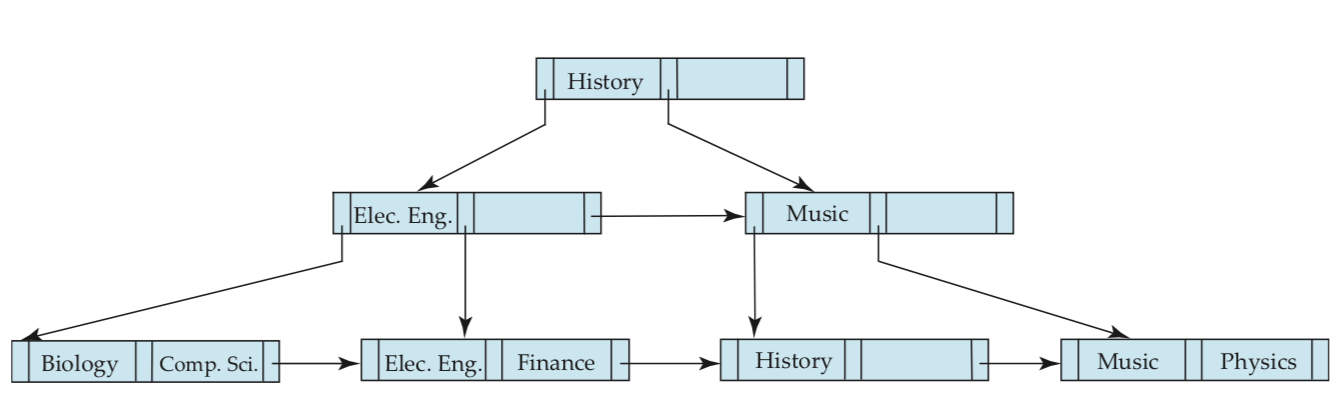
\includegraphics[width=0.9\textwidth]{images/b-link1}
	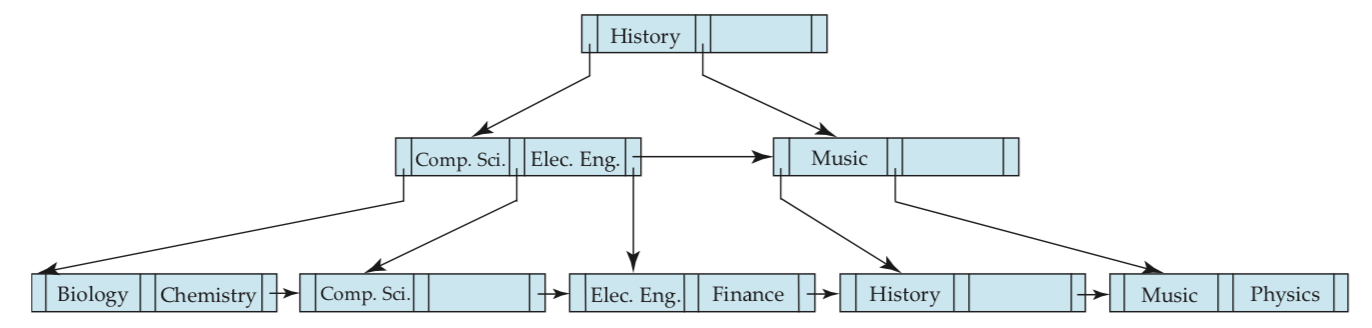
\includegraphics[width=0.9\textwidth]{images/b-link2}\\
	Insertion of ``Chemistry'' into a B-Link tree (before above, after below).~\cite{dsc}
\end{center}

So, running through the example: the insertion operation runs and it finds the destination where ``Chemistry'' should be inserted, which results in splitting the node  at the bottom left and the creation of a new one.  

Now let's see what happens if there is a lookup while this is going on at this point. The lookup gets blocked at the bottom-left leaf node because it is exclusively locked by the insertion. The lookup holds no locks at this point.

The insertion operations complete and relocks the parent node in exclusive mode, completing the insertion. This completely screws up the lookup operation because it is now holding a pointer to the wrong node. That's okay, because the lookup can start moving to the right through the sibling nodes until it finds the correct one. That seems a little bit painful, but it does mean it will succeed.

If instead of a split there was a coalescence, a lookup might be left holding the pointer to a node that no longer exists. That's okay, this lookup just needs to restart from the beginning. It's not ideal, but it does happen. To reduce the amount of times this happens, we might try to leave some nodes uncoalesced even when that would be the normal procedure; this breaks the rules about B-Trees, but it might be very brief if there are many more insertions than deletions.

\paragraph{Key-Value Locking.} Key-value locking allows locking individual key values allowing other operations to take place on values within the same leaf node and potentially increasing concurrency. The problem is that we could still have the phantom phenomenon, so the strategy of \textit{next key locking} is employed: not only lock the keys that are in the range/search result but also whichever one is next~\cite{dsc}. This prevent something from being inserted, altered, or deleted inside the search range. 

\bibliographystyle{alphaurl}
\bibliography{356}


\end{document}
